\documentclass[final,bibliography=totocnumbered]{include/seminar}

% Some packages have already been loaded by the seminar class.
% See include/seminar.cls for a list

\usepackage{todonotes}

\usepackage[backend=bibtex]{biblatex}
\usepackage{amsfonts}
\usepackage{amsmath}
\usepackage{mathtools}
\usepackage{ntheorem}
\usepackage{relsize}

\usepackage{tikz}
\usepackage{tikz-3dplot}
\usepackage{pgfplots}

\usepackage{algorithm}
\usepackage{algorithmic}
\usepackage{caption}
\usepackage{microtype}

\bibliography{literatur.bib}

\graphicspath{{./figures/}}

\clubpenalty=10000
\widowpenalty=10000

% Mark overfull hboxes
\overfullrule=1mm

\setlength\parindent{0pt}
\setlength{\headheight}{15pt}
\linespread{1.1}

\newcommand{\mR}{\ensuremath{\mathbb{R}}}
\newcommand{\mRn}{\ensuremath{\mathbb{R}^n}}
\newcommand{\mRnn}{\ensuremath{\mathbb{R}^{n \times n}}}
\newcommand{\mRd}{\ensuremath{\mathbb{R}^d}}

\newcommand{\Ltwo}{\ensuremath{{L^2(\Omega)}}}
\newcommand{\Hone}{\ensuremath{{H^1(\Omega)}}}
\newcommand{\Honez}{\ensuremath{{H^1_0(\Omega)}}}
\newcommand{\Hdual}{\ensuremath{{H^{-1}(\Omega)}}}

\newcommand{\mA}{\ensuremath{\mathcal{A}}}
\newcommand{\mAi}{\ensuremath{\mathcal{A}}^{-1}}
\newcommand{\mAh}{\ensuremath{\mathcal{\tilde{A}}}}
\newcommand{\mAhi}{\ensuremath{\mathcal{\tilde{A}}}^{-1}}
\newcommand{\mI}{\ensuremath{\mathcal{I}}}

\newcommand{\GP}{Gross-\allowbreak Pi\-taev\-skii}
\newcommand{\GPEnergy}{Gross-Pitaevskii Energiefunktional}

\theoremstyle{break}
\newtheorem{theorem}{Theorem}[section]
\newtheorem{corollary}{Korollar}[theorem]
\newtheorem{lemma}{Lemma}[theorem]
\newtheorem{definition}{Definition}[section]

\begin{document}

\Title{Inverse Iteration}
\Studiengang{Bachelor Mathematik}

\Prof{Prof. Dr. Tatjana Stykel}
\Chair{Lehrstuhl für Numerische Mathematik}

\Author{Max Grübmeyer}
\date{Ausarbeitung zum Vortrag am 11.07.2025}

\subject{Seminar zum Thema Eigenwertprobleme mit Eigenvektor-Nichtlinearitäten}

\makeAuthor
\makeTitle
\maketitle

\begin{abstract}

\setlength\parindent{0pt}
\setlength{\headheight}{15pt}
\linespread{1.1}

\section*{Kurzfassung}

Viele Probleme in der Physik, den Natur- und Ingenieurswissenschaften, aber
auch aus der Data Science lassen sich als
Eigenwertprobleme mit Eigenvektor-Nichtlinearitäten formulieren.
Dies ist eine Generalisierung des klassischen Eigenwertproblems aus der
Linearen Algebra,
in dem Lösungen
$v \in \mRn$ der Gleichung
$A(v)v = \lambda v$ für $A: \mRn \rightarrow \mRnn$ und ein $\lambda \in \mR$
gesucht werden.

Einen Ansatz, diese Probleme numerisch zu lösen, bietet die Inverse Iteration, auch
    A-Methode genannt, welche ursprünglich in \cite{intro} vorgestellt wurde.
Diese stellt eine Generalisierung der klassischen Inversen Iteration aus der
numerischen Linearen Algebra dar.

\medskip

Diese Arbeit ist die Ausarbeitung
zum Vortrag vom $11.07.2025$, welcher zu großen Teilen auf \cite{main} basiert.
Anhand des \GP{} Eigenwertproblems soll die A-Methode motiviert
und deren grundlegende Konvergenzeigenschaften skizzenhaft
abgehandelt werden.
Ebenso soll untersucht werden, wie die Methode auf Shifts reagiert.
Das Ganze wird abschließend mit numerischen Experimenten untermauert.

\end{abstract}

\thispagestyle{empty}

\newpage

\tableofcontents

\newpage

\section{Einleitung}

Wird ein verdünntes Gas von Bosonen auf Temperaturen nahe des absoluten Nullpunkts
heruntergekühlt, so tritt ein besonderes quantenmechanisches Phänomen auf.
Ein makroskopische Anteil der Teilchen kondensiert in den Grundzustand, es
entsteht ein Bose-Einstein-Kondensat. In diesem Zustand lässt sich das Verhalten
des gesamten Systems durch eine einzige, makroskopische Wellenfunktion beschreiben.

Besonders interessant ist hierbei der Grundzustand - der niedrigstenergetische
Zustand, welches das System einnehmen kann - sowohl im Hinblick auf das äußere
Potential, als auch auf die Wechselwirkungen zwischen den Teilchen.

Das populärste mathematische Modell, um dieses Problem zu untersuchen, und
den Grundzustand zu finden, ist hierbei durch das \GP{} Eigenwertproblem gegeben.

\medskip

Seien im Folgenden

\begin{itemize}
    \item $\Omega \in \mRd$ ein beschränktes und offenes Gebiet der Dimension $d = 1,2,3$.
		Die Dimension wird in dieser Ausarbeitung nicht behandelt, ist aber für
		benötigte Sobolev-Einbettungen von Bedeutung.
    \item $V \in L^\infty(\Omega)$ ein Potential, welches für fast alle $x \in
		\Omega$ nicht-negativ ist.
    \item $\beta \geq 0$ eine reellwertige Konstante, welche die Abstoßung der
		Teilchen beschreibt.
\end{itemize}

dann ist das {\GPEnergy} definiert durch

\begin{align}\label{GPE}
    E(v) \coloneq \frac{1}{2} \mathlarger{\int}_{\Omega} \mathsmaller{\frac{1}{2}\vert \nabla v \vert ^2 + V \vert v \vert ^2 + \frac{\beta}{2}\vert v \vert ^4} \,dx
\end{align}

Der natürliche Funktionenraum dieses Problems ist der Sobolevraum $\Hone$, der Raum der $\Ltwo$-Funktionen,
dessen erste schwache Ableitungen wieder in $\Ltwo$ liegen.
Zudem lässt sich dieser in $L^4(\Omega)$ einbetten, weshalb (\ref{GPE}) für
jede Funktion aus $\Hone$ wohldefiniert ist.
Wir fordern zudem noch eine Nullrandbedingung, dieser eingeschränkte Raum
wird im Folgenden mit $\Honez$ notiert, sein Dualraum ist $\Hdual$.

\medskip

Gesucht ist nun ein $u \in \Honez$ mit $\Vert u \Vert_\Ltwo = 1$, welches das {\GPEnergy} minimiert.
Da (\ref{GPE}) schwach unterhalbstetig und von unten durch $0$ beschränkt ist,
exisiert ein Minimum.
Aus der Ungleichung $\vert\nabla\vert v \vert\vert \leq \vert\nabla v\vert$
folgt, dass wenn $u$ ein Minimierer ist, auch $\pm \vert u \vert$ ein Minimierer
sein muss.
Darauf aufbauend kann gezeigt werden, dass der Minimierer entweder strikt
positiv oder strikt negativ sein muss - und, dass er bis auf sein Vorzeichen
eindeutig bestimmt ist.\cite{sign}

\medskip

Eine Umformulierung von (\ref{GPE}) mithilfe der Euler-Lagrange Gleichungen
liefert uns die alternative Formulierung

\begin{align}\label{Euler-Lagrange}
    &\langle E'(u), v \rangle = \lambda(u,v)_\Ltwo &\forall v \in \Honez
\end{align}

wobei $E'$ die Fréchet-Ableitung von $E$ an der Stelle $u$, $\lambda > 0$
und $\langle \cdot,\cdot \rangle$ die kanonische duale Paarung ist.
Eine Lösung $u \in \Honez$ von (\ref{Euler-Lagrange}) ist genau dann eine Lösung von (\ref{GPE}),
wenn $\lambda > 0$ minimal ist. Die Fréchet-Ableitung kann wie folgt berechnet werden:

\begin{align}
    \langle E'(u), v\rangle = \frac{1}{2}(\nabla u, \nabla v)_\Ltwo
    + (Vu, v)_\Ltwo + \beta(\vert u \vert^2 u, v)_\Ltwo
\end{align}

Parametrisiert man weiter landet man bei $\mA_z: \Honez \rightarrow \Hdual$ mit

\begin{align}
    \langle\mA_z u, v\rangle = \frac{1}{2}(\nabla u, \nabla v)_\Ltwo
    + (Vu, v)_\Ltwo + \beta(\vert z \vert^2 u, v)_\Ltwo
\end{align}

Gesucht ist also das $u \in \Honez$ mit minimalem $\lambda > 0$, sodass

\begin{align}\label{EVP}
    \langle A_u, u, \cdot\rangle = \lambda(u, \cdot)_\Ltwo = \lambda\mI u
\end{align}

wobei $\mI: \Honez \rightarrow \Ltwo', u \mapsto (u, \cdot)_\Ltwo$ die Inklusion
ist.
Da $\mA_u$ eine koerzive, symmetrische Bilinearform ist, garantieren uns
Standardresultate aus der Lösungstheorie partieller Differentialgleichung,
dass eine abzählbare Anzahl an Eigenwerten

\begin{align*}
    0 < \lambda_1 < \lambda_2 \leq \lambda_3 \leq ... \rightarrow \infty
\end{align*}

existiert. Die dazugehörigen Eigenfunktionen spannen den Raum auf,
der erste Eigenwert $\lambda_1$ ist einfach und es existiert
ein Spectral Gap, d.h. $\frac{\lambda_1}{\lambda_2} < 1$.\cite{evans}

\section{Die Inverse Iteration}

Um den kleinsten Eigenwert eines Operators mit Spectral Gap zu berechnen,
gibt es in der numerischen Linearen Algebra den Algorithmus der Inversen Iteration.
Dieser soll nun im Folgenden auf nichtlineare Eigenwertprobleme erweitert werden.
Die Idee ist es durch $A(v)$ zu linearisieren, der Rest funktioniert analog.
Das Resultat ist der folgende Algorithmus zur Inversen Iteration - auch A-Methode genannt:

\begin{algorithm}[H]
    \caption{Inverse Iteration (A-Methode)}
    \begin{algorithmic}[1]
        \STATE $u^0 \in \Honez$
        \FOR{$n=0$ to $Konvergenz$}
        \STATE $u^{n+1} = \frac
        {\mA_{u^n}^{-1} u^n}
        {\Vert \mA_{u^n}^{-1} u^n \Vert}$
        \ENDFOR
    \end{algorithmic}
\end{algorithm}

wobei in unserem Fall $\mA_v^{-1} \coloneq \mAh_v^{-1}\mI$ gilt.

\section{Lokale Konvergenz}

Will man die Konvergenz dieses Algorithmus untersuchen, so liefert der Banach'sche
Fixpunktsatz kein Resultat. Die Iteration ist zwar eine Selbstabbildung in einem
vollständigen metrischen Raum, aber im Allgemeinen nicht kontraktiv.
Das benötigte Werkzeug wird uns in Form des folgenden Theorems bereitgestellt:

\begin{theorem}[Theorem von Ostrowski]
    Sei $u \in \Honez$ und $\phi: \Honez \rightarrow \Honez$ mit Fréchet-Ableitung $\phi'(u)$ an der Stelle $u$.
    Hat diese Spektralradius $\rho \coloneq \rho(\phi'(u)) < 1$,
    dann existiert offene $H^1$ Umgebung $S$ von $u$, sodass die Fixpunktiteration
    \begin{align*}
        u^{n+1} = \phi(u^n)
    \end{align*}
    für alle $u^0 \in S$ gegen $u$ konvergiert.

    \medskip

    Genauer gilt dann: Für jedes $\varepsilon > 0$ existiert eine offene
    Umgebung $S_\varepsilon$ von $u$ und eine Konstante $C_\varepsilon > 0$:
    \begin{align*}
        \Vert u^n - u \Vert_\Hone \leq C_\varepsilon \vert \rho + \varepsilon \vert^n \Vert u^0 - u \Vert_\Hone\;\; \forall u^0 \in S_\varepsilon, n \geq 1
    \end{align*}
\end{theorem}
\cite{ostrowski-original}
\cite{ostrowski-improved}

\medskip

Berechnet man nun die Fréchet-Ableitung $\phi'$ von
$\phi(v) \coloneq \frac{\mAi_v v}{\Vert \mAi_v v \Vert}$ an der Stelle
des Minimums $u$, dann lässt sich zeigen,
dass diese tatsächlich den Spektralradius
$\rho = \rho(\phi'(u)) < 1$ besitzt.

Genauer gilt folgendes:
\begin{align}
    \rho = \underset{i}{\mathrm{sup}} \vert \mu_i \vert
    \leq (1 - \delta) \frac{\lambda_1}{\lambda_2} < 1
\end{align}

wobei $\delta \in (0, 1)$ eine Konstante ist, die aus den Abschätzungen herausfällt
und $\mu_i$ die Eigenwerte der Fréchet-Ableitung $\phi'$ an der Stelle $u$ sind.

Somit garantiert uns Ostrowski's Theorem lokale Konvergenz für
$\varepsilon < \delta\frac{\lambda_1}{\lambda_2}$.

\section{Globale Konvergenz}

\subsection{Ein Gradientenflussverfahren}

Um die globale Konvergenz unseres Verfahrens zu untersuchen betrachten wir
das Problem aus einem anderen Blickwinkel. Gesucht ist ein Minimierer $u \in \Honez$
des \GPEnergy s unter der Nebenbedingung $\Vert u \Vert_\Ltwo = 1$.
Dies ist also ein riemannsches Optimierungsproblem auf der Mannigfaltigkeit
$\mathbb{S} \coloneq \{v \in \Honez\vert\: \Vert v \Vert_\Ltwo = 1\}$.

\medskip

Wir konstruieren nun ein Gradientenflussverfahren auf $\mathbb{S}$,
welches ursprünglich in \cite{flow} vorgestellt und untersucht wurde.
Gegeben ein $u_0 \in \mathbb{S}$ wird ein
$z \in C^1([0, \infty];\mathbb{S})$ mit $z(0) = u_0$ gesucht, welches
für alle $t > 0$ die folgende Differentialgleichung erfüllt:

\begin{align}
    &z'(t) = -z(t) + \gamma(z(t))\mAi_{z(t)}z(t)
    &\text{wobei } \gamma(z) \coloneqq (\mAi_zz, z)_\Ltwo^{-1}
\end{align}

Dieses Problem ist wohl gestellt und man kann zwei wichtige Eigenschaften zeigen:
\begin{align}\label{spherenorm}
    \frac{1}{2}\frac{d}{dt}\Vert z(t) \Vert^2 = 0
\end{align}
und
\begin{align}\label{sphereway}
    - \frac{d}{dt}E(z(t)) \geq 0
\end{align}
wobei $E$ das {\GPEnergy} ist.

\medskip

(\ref{spherenorm}) bedeutet, dass die Norm nicht zeitabhängig ist. Ist $u_0 \in \mathbb{S}$, so
wird auch $z(t)$ für alle $t > 0$ wieder in $\mathbb{S}$ liegen.
$z$ beschreibt also eine zeitabhängige Bewegung auf der $\Ltwo$-Sphäre $\mathbb{S}$.
(\ref{sphereway}) ist äquivalent dazu, dass die Energie nach der Zeit abnimmt. Zu erwarten
ist also eine Konvergenz gegen das Minimum (oder generell, einen kritischen Punkt).

\def\myr{3}
\tdplotsetmaincoords{65}{125}

\begin{figure}
    \centering
    \begin{tikzpicture}
        \coordinate (O) (0,0);
        \draw[thick, ball color=gray, opacity=0.3, draw opacity=1] 
            (O) circle[radius={\myr}];
    
        \begin{scope}[tdplot_main_coords, rotate=-10]
            \begin{scope}[canvas is xy plane at z=0]  
                % Back half circle (dashed)
                \draw[dashed] (\tdplotmainphi:\myr) 
                    arc[start angle={\tdplotmainphi}, 
                        end angle={\tdplotmainphi+180}, 
                        radius={\myr}] coordinate (R);
                % Front half circle (solid) + BL
                \draw[thick] (\tdplotmainphi:\myr) 
                    arc[start angle={\tdplotmainphi}, 
                        end angle={\tdplotmainphi-180}, 
                        radius={\myr}] coordinate (L);
            \end{scope}
    
            \begin{scope}[canvas is yz plane at x=0]
                \draw[dashed] (\tdplotmainphi:\myr) 
                    arc[start angle={\tdplotmainphi}, 
                        end angle={\tdplotmainphi+180}, 
                        radius={\myr}];
                \draw[thick] (\tdplotmainphi:\myr) 
                    arc[start angle={\tdplotmainphi}, 
                    end angle={\tdplotmainphi-180}, 
                    radius={\myr}];
            \end{scope}
            
            \begin{scope}[canvas is xz plane at y=0]
                \draw[dashed] (\tdplotmainphi:\myr) 
                    arc[start angle={\tdplotmainphi}, 
                        end angle={\tdplotmainphi+180}, 
                        radius={\myr}];
                \draw[thick] (\tdplotmainphi:\myr) 
                    arc[start angle={\tdplotmainphi}, 
                        end angle={\tdplotmainphi-180}, 
                        radius={\myr}];
                % Axis
            \end{scope}
    
            \begin{scope}
                % Parameter für den Pfad
                \def\waveamp{0.2}
                \def\wavemult{8}
                \def\maxangle{64}
    
                % Startpunkt speichern
                \pgfmathsetmacro{\thetaStart}{0}
                \pgfmathsetmacro{\zshiftStart}{\waveamp*sin(\wavemult*\thetaStart)}
                \pgfmathsetmacro{\xStart}{\myr*cos(\thetaStart)}
                \pgfmathsetmacro{\yStart}{\myr*sin(\thetaStart)}
    
                % Endpunkt speichern
                \pgfmathsetmacro{\thetaEnd}{\maxangle}
                \pgfmathsetmacro{\zshiftEnd}{\waveamp*sin(\wavemult*\thetaEnd)}
                \pgfmathsetmacro{\xEnd}{\myr*cos(\thetaEnd)}
                \pgfmathsetmacro{\yEnd}{\myr*sin(\thetaEnd)}
    
                % Pfad zeichnen
                \foreach \i in {0,...,\numexpr\maxangle-1} {
                    \pgfmathsetmacro{\thetaA}{\i}
                    \pgfmathsetmacro{\thetaB}{\i + 1}
                    \pgfmathsetmacro{\zshiftA}{\waveamp*sin(\wavemult*\thetaA)}
                    \pgfmathsetmacro{\zshiftB}{\waveamp*sin(\wavemult*\thetaB)}
                    \pgfmathsetmacro{\xA}{\myr*cos(\thetaA)}
                    \pgfmathsetmacro{\yA}{\myr*sin(\thetaA)}
                    \pgfmathsetmacro{\xB}{\myr*cos(\thetaB)}
                    \pgfmathsetmacro{\yB}{\myr*sin(\thetaB)}
                    \draw[red, thick] 
                        (\xA,\yA,\zshiftA) -- (\xB,\yB,\zshiftB);
                }
    
                % Startpunkt markieren
                \filldraw[fill=red, draw=black] 
                    (\xStart,\yStart,\zshiftStart) circle[radius=2pt] 
                    node[above right] {$u_0$};
    
                % Endpunkt markieren
                \filldraw[fill=green!70!black, draw=black] 
                    (\xEnd,\yEnd,\zshiftEnd) circle[radius=2pt] 
                    node[below right] {$u$};
            \end{scope}
        \end{scope}
    \end{tikzpicture}
	\caption{Optimierungsproblem auf der Einheitssphäre $\mathcal{S}_2$. Ein zeitabhängiger Weg
    vom Startpunkt $u_0$ zum Minimum $u$ - visualisiert im Dreidimensionalen.\cite{blueball}}
\end{figure}

\subsection{Die gedämpfte Inverse Iteration}

Anhand dieser Differentialgleichung wird nun die gedämpfte Inverse Iteration
konstruiert.
Diskretisiert man $z'(t) \approx \frac{z^{n+1} - z^n}{\tau_n}$ erhält man folgendes:
\begin{align*}
    &\frac{z^{n+1} - z^n}{\tau_n} = -z^n + \gamma(z^n)\mAi_{z^n}z^n
    &\text{oder aufgelöst } z^{n+1} = (1 - \tau_n)z^n + \tau_n\gamma(z^n)\mAi_{z^n}z^n
\end{align*}

Da die Normalisierung durch die Diskretisierung verloren gehen kann, wird zusätzlich
noch in jedem Schritt normiert. Dadurch bekommen wir das Verfahren der
gedämpften Inversen Iteration:

\begin{algorithm}[H]
    \caption{Gedämpfte Inverse Iteration}
    \begin{algorithmic}[1]
        \STATE $u^0 \in \Honez$
        \FOR{$n=0$ to $Konvergenz$}
        \STATE $u^{n+1} = \frac
        {(1-\tau_n)u^n + \tau_n\gamma(u^n)\mA_{u^n}^{-1} u^n}
        {\Vert(1-\tau_n)u^n + \tau_n\gamma(u^n)\mA_{u^n}^{-1} u^n\Vert}$
        \ENDFOR
    \end{algorithmic}
\end{algorithm}

Die Konvergenz dieser Methode hängt natürlich von der Wahl der Parameter
$\tau_n$ ab. Offensichtlich machen nur $\tau_n > 0$ Sinn, ebenso kann man zeigen,
dass die Iteration zwangsläufig für $\tau_n > 2$ divergieren muss.
Das folgende Theorem liefert eine noch schärfere Aussage über das Konvergenzverhalten
der gedämpften Inversen Iteration.

\begin{theorem}[Theorem über die Globale Konvergenz]
    Es exisitiert ein $\tau_{crit} \in (0,2)$, sodass die gedämpfte Inverse
    Iteration mit jeder Folge $(\tau_n)_{n \in \mathbb{N}}$, die
    \begin{align*}
        0 < \tau_n < \tau_{crit}
    \end{align*}
    erfüllt für alle Startwerte $u^0 \in \Honez$ mit $\Vert u^0 \Vert = 1$
    und $u^0 > 0$ konvergiert.

    Insbesondere gilt dies für $\tau_{crit} = 2(1 + \frac{\lambda_1}{\lambda_2})^{-1} \in (1, 2)$.
\end{theorem}

Da die gedämpfte Inverse Iteration für alle $\tau_n < \tau_{crit}$ konvergiert,
stellt sich die Frage, für welche $\tau_n$ lokal die beste Konvergenzrate
errreicht wird.
Tatsächlich konvergiert das Verfahren für alle $\tau_n$ mit $0 < \tau_n < 2(1 + \frac{\lambda_1}{\lambda_2})^{-1} $ linear,
die beste Konvergenzrate wird aber für $\tau_n = 1$, also die ungedämpfte Version
des Verfahrens, erreicht.

\medskip

Das Verfahren kann also in zwei Phasen aufgeteilt werden.
In der ersten Phase werden die $\tau_n$ in jedem Schritt adaptiv gewählt,
um möglichst schnell in eine Umgebung der optimalen Lösung $u$ zu kommen.
Anschließend wird in der zweiten Phase die Dämpfung
ausgeschaltet ($\tau_n = 1$), um
innerhalb der Umgebung möglichst schnell gegen $u$ zu konvergieren.

\medskip

Die Dämpfungsparameter $\tau_n \in (0, 2)$ können in der ersten Phase als Lösung des
folgenden Minimierungsproblems gewählt werden

\begin{align*}
    \tau_n = \mathrm{arg min}
    \mathlarger{\mathlarger{\mathlarger{\{}}}
    E\big(\frac{(1 - \tau_n)u^n + \tau_n\gamma(u^n)\mA_{u^n}^{-1}(u^n)}
    {\Vert(1 - \tau_n)u^n + \tau_n\gamma(u^n)\mA_{u^n}^{-1}(u^n)\Vert}\big)
    \mathlarger{\mathlarger{\mathlarger{\}}}}
\end{align*}

wobei $E$ das {\GPEnergy} ist. Gewählt wird also in jedem Schritt
das $\tau_n$, welches die Energie des nächsten Schrittes minimiert.
Dieses Minimierungsproblem wird klassischerweise mithilfe von Liniensuchverfahren
gelöst, eine mögliche Implementierung liefern \cite{flow} und \cite{flow_min}.

\medskip

Da in jedem Schritt das $\tau_n$ gewählt wird, welches die Energie im
nächsten Schritt minimiert,
lässt sich durchaus von einem Greedy Algorithmus sprechen.
Deshalb ist anzumerken, dass dieser zwar für jeden Schritt das beste $\tau_n$
wählt, dies aber nicht zwangsläufig über mehrere Schritte hinweg die beste
Wahl sein muss.

\section{Shifts}

Die Konvergenzrate der klassischen Inversen Iteration kann durch einen geschickten
Shift $\sigma \in \mR$ verbessert werden, die Konvergenzrate ist dann
$\frac{\lambda_1 - \sigma}{\lambda_j - \sigma}$ für ein $j \neq 1$.
Diese Herangehensweise ist allerdings bei der Generalisierung der Inversen
Iteration im Allgemeinen nicht zielführend.
Gegeben die Iterationsvorschrift
\begin{align}
    \phi(u^n) \coloneq u^{n+1} = \frac{(\mAi_{u^n} - \sigma I)u^n}{(\Vert\mAi_{u^n} - \sigma I)u^n\Vert}
\end{align}
wobei $\sigma \in \mR$ der Shift und $I$ die Identität auf $\Honez$ ist,
dann ist die Konvergenzrate dieses Verfahrens vom Spektralradius $\rho \coloneq \rho(\phi'(u))$
der Fréchet-Ableitung $\phi'$ an der Stelle der optimalen Lösung $u$ abhängig.

Berechnet man nun den Spektralradius der Fréchet-Ableitung des geshifteten
Verfahren, so lässt sich folgendes Resultat zeigen:

\begin{align}
    \rho = \underset{i}{\mathrm{sup}} \vert \mu_i \vert
    = \vert \lambda_1 - \sigma \vert \underset{i}{\mathrm{sup}}
    \frac{\vert((1-2\frac{\beta}{\lambda_1 - \sigma}\vert u\vert^2)v_i,
    (\mAi_u - \sigma I)v_i)_\Ltwo \vert}
    {\Vert v_i \Vert^2}
\end{align}

wobei $\mu_i \in \mR$ den zum Eigenvektor $v_i \in \Honez$ zugehörigen Eigenwert darstellt.

Das Problem ist hierbei, dass man für möglichst schnelle Konvergenz den Term
$\vert \lambda_1 - \sigma \vert$ minimieren möchte - hierdurch riskiert man
aber gleichzeitig einen möglichen Blow-up des Terms $(1 - 2 \frac{\beta}{\lambda_1 - \sigma}\vert u \vert^2)$.

Dies liefert die Begründung dafür, wieso die geshiftete Version der A-Methode
im Allgemeinen nur schlecht - oder gar nicht - für das \GP{} Eigenwertproblem
funktioniert. Numerische Experimente untermauern dies (vgl. z.B. \cite{intro}).

\section{Numerische Simulation}

Um das ganze numerisch zu simulieren, muss das \GP{} Eigenwertproblem
erst diskretisiert werden. Hierzu wird $A$ wie folgt konstruiert
\begin{align}
    A(v) = L_N + M_V + \tilde{A}(v)
\end{align}

wobei Lösungen der Form $A(v)v = \lambda v$ mit minimalem $\lambda$ gesucht werden.
Hierbei ist $L_N$ der diskretisierte zweidimensionale Laplace-Operator, d.h.
$L_N = D_2 \otimes I + I \otimes D_2$, wobei
\begin{align}
    D_2 = \frac{1}{h^2}
    \begin{bmatrix}
        2 & -1 & 0 & \cdots & 0 \\
        -1 & 2 & -1 & \cdots & 0 \\
        0 & -1 & 2 & \cdots & 0 \\
        \vdots & \vdots & \vdots & \ddots & -1 \\
        0 & 0 & 0 & -1 & 2
    \end{bmatrix}
\end{align}

der eindimensionale Laplace, $\otimes$ das Kronecker-Produkt und $h$ die
Schrittweite ist.

\medskip

Als Potential wurde das harmonische Potential gewählt, welches durch
$M_V$ mit ${M_V}_{ij} = \frac{1}{2}(x_i^2 + y_j^2)$
dargestellt wird. Die Nichtlinearität kommt durch die Interaktion der
Teilchen mit
$\tilde{A}(v) = \frac{1}{h^2}\beta\:\texttt{diag}(\vert v \vert)^2$.

\medskip

Das Problem wird auf der Domäne $[-8,8]^2 \subset \mR^2$ betrachtet,
wobei diese durch $200$ äquidistante Schritte diskretisiert wurde.
Die Experimente wurden mit verschiedenen Nichtlinearitätsparametern
$\beta = 10^{-1}, 10^0, 10^1, 10^2, 10^3$ durchgeführt.

\begin{figure}
    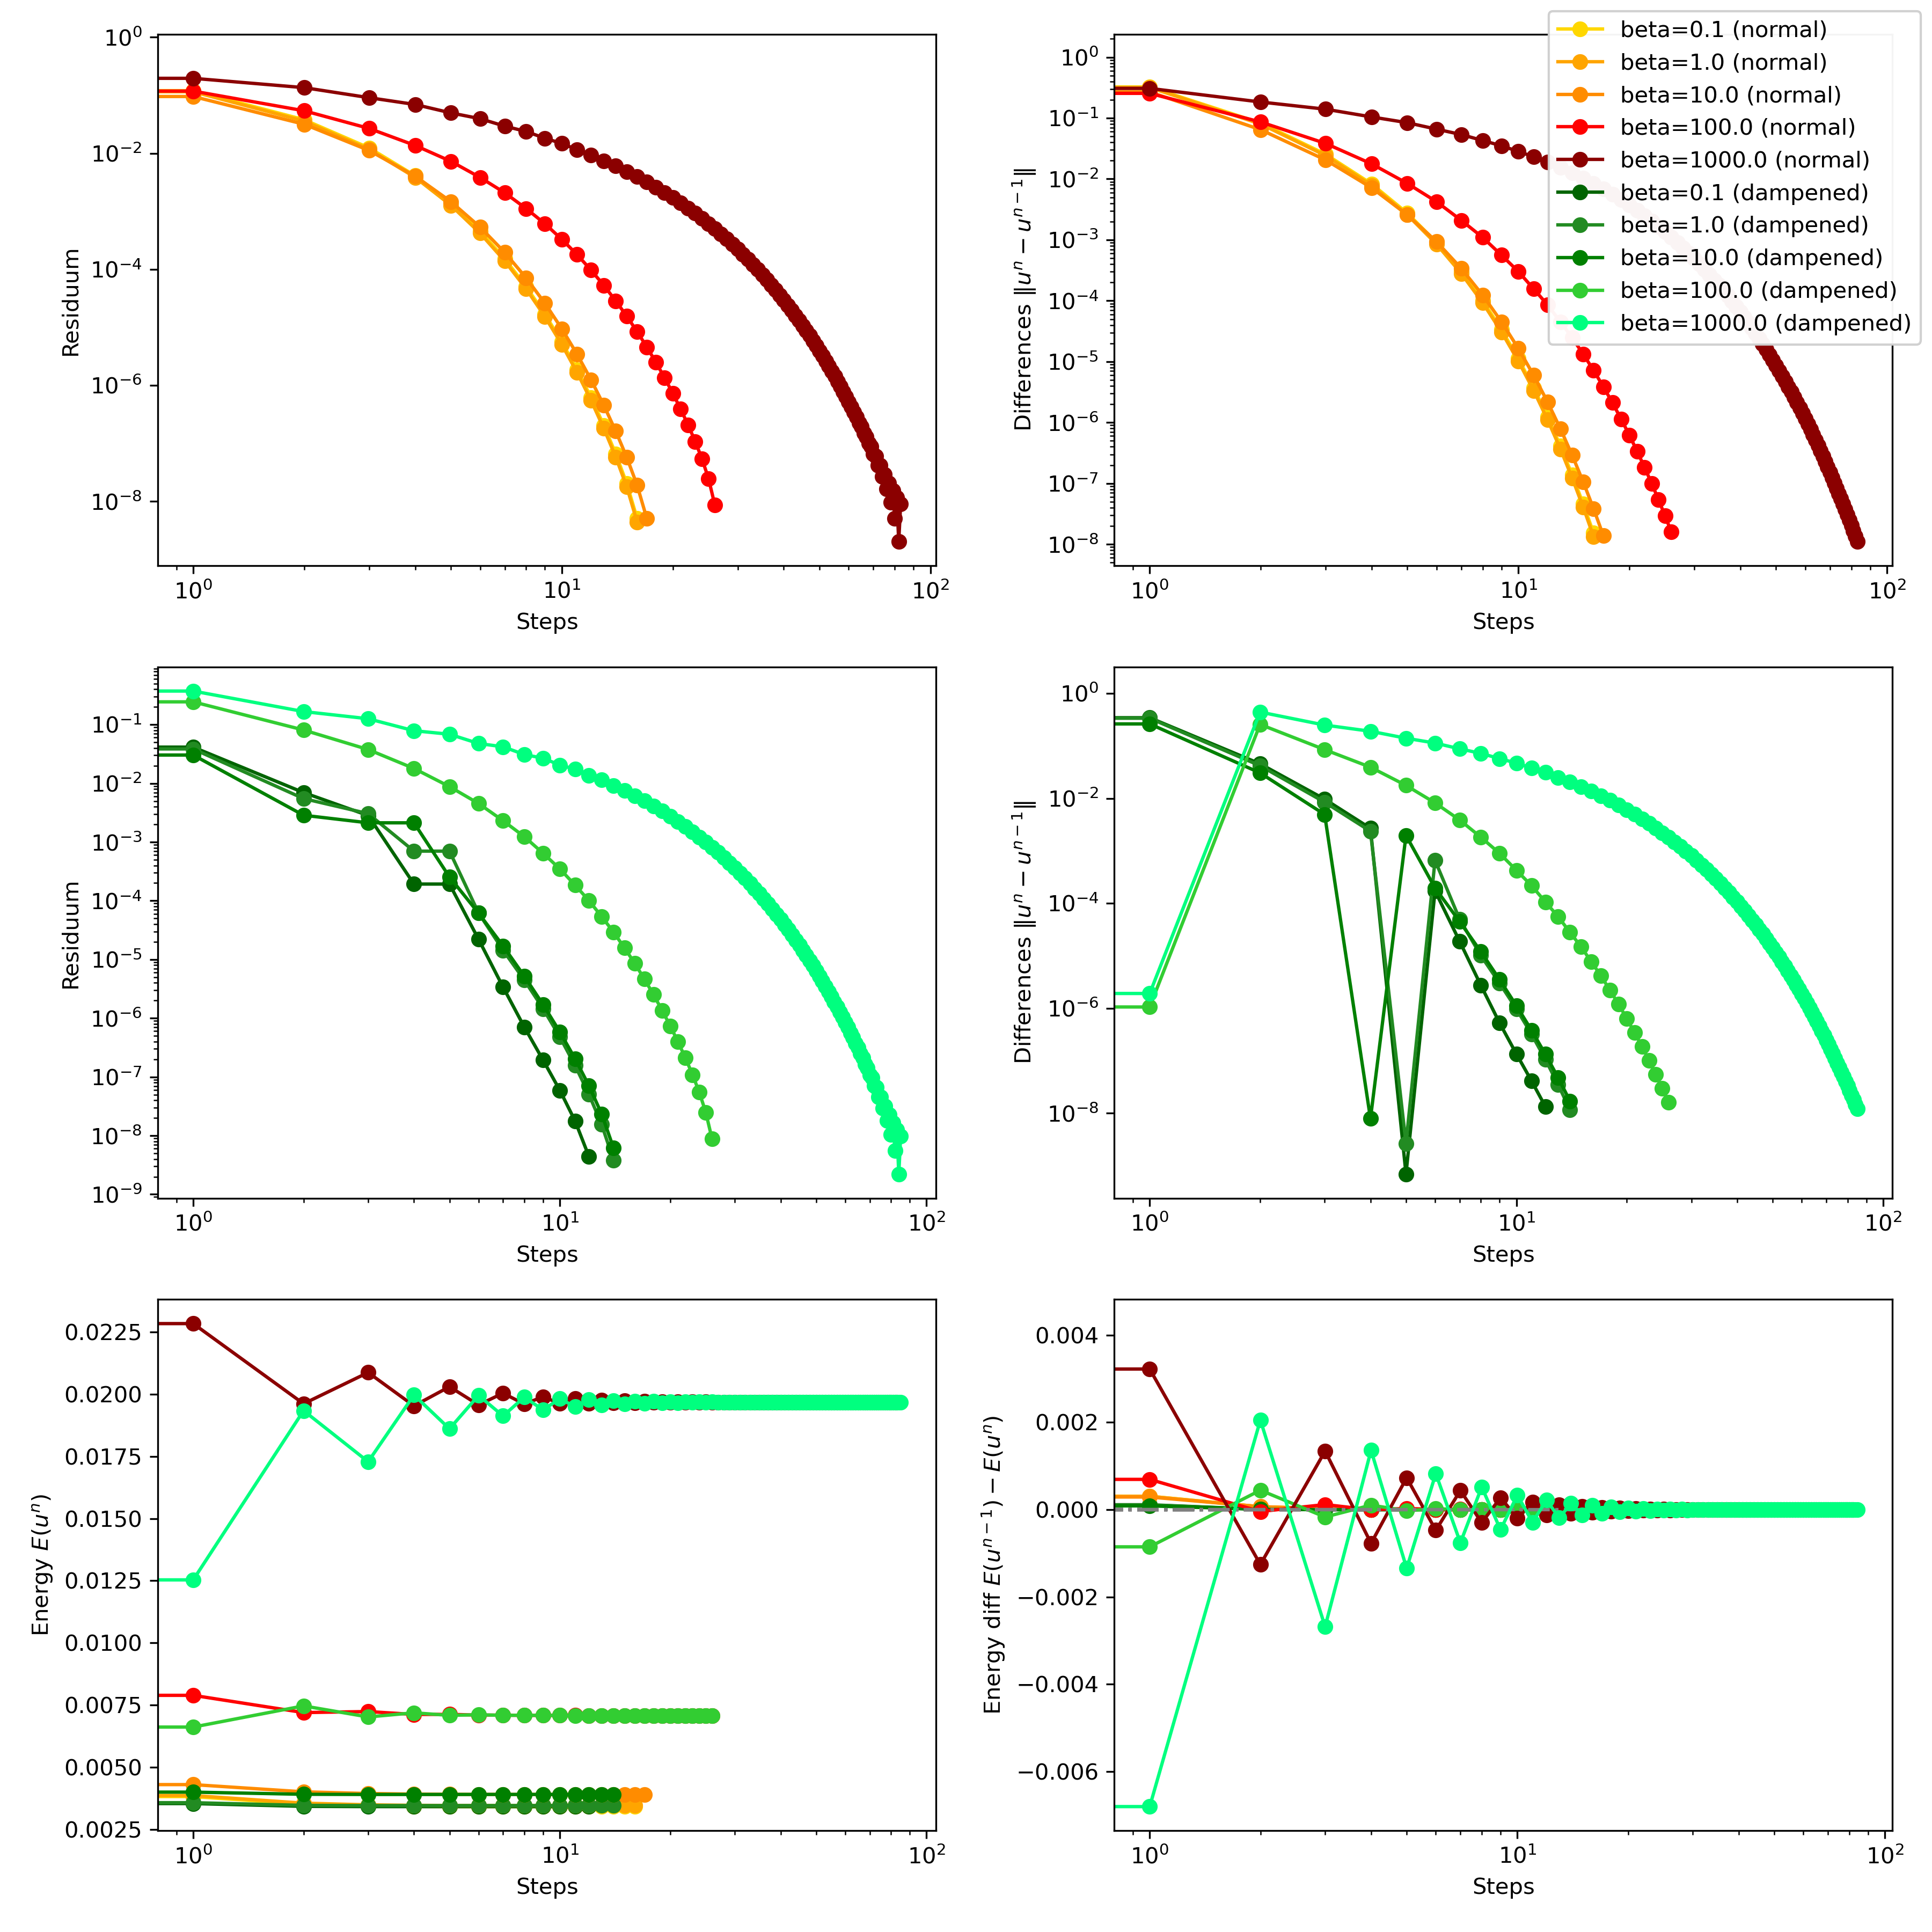
\includegraphics[width=\textwidth]{../img/gpe-inverse-iteration-comparision.png}
    \caption{Abbildungen des Verhaltens sowohl der ungedämpften
    (obere Reihe) als auch der gedämpften Version (mittlere Reihe) der A-Methode.
    In der letzten Reihe wird der Energieverlauf der beiden Verfahren verglichen.}
\end{figure}

In jedem getesteten Szenario reduziert die Dämpfung die Anzahl der benötigten
Schritte im Vergleich zum ungedämpften System.
Um die optimalen Dämpfungsparameter $\tau_n$ zu wählen, wurde auf die Bibliotheksfunktion
\textit{scipy.optimize.minimize\_scalar} zurückgegriffen.
Es ist möglich, dass die Konvergenzgeschwindigkeit der gedämpften Inversen Iteration
durch einen besseren Minimierer erheblich beschleunigt werden könnte.
Interessant ist auch der Energieverlauf. Während die gedämpfte Variante in jedem
Schritt ein niedrigeres Energieniveau erreicht, kann es vorkommen, dass die
ungedämpfte Variante in manchen Schritten auf ein höheres Energieniveau sprint.
Dies tritt besonders bei Problemen mit größerer Nichtlinearität auf.

\begin{table}
\begin{center}
\begin{tabular}{ | p{8em} | r | r | r | r | r |}
	\hline
	& $\beta=0.1$ & $\beta=1.0$ & $\beta=10.0$ & $\beta=100.0$ & $\beta=1000.0$ \\
	\hline
	A-Methode & 18 & 18 & 20 & 35 & 124 \\
	--- gedämpft & 15 & 15 & 18 & 34 & 99 \\
	--- geshifted & 8 & 8 & 18 & 84 & N/A \\
	\hline
\end{tabular}
\caption{Konvergenzverhalten der Verfahren im Vergleich. Die Spalten beinhalten
die Anzahl der Schritte bis zur Konvergenz für gegebene Nichtlinearität $\beta$.
N/A signalisiert, dass das Verfahren in 200 Schritten nicht konvergiert ist.}
\label{tab:conv}
\end{center}
\end{table}

\medskip

Die geshiftete A-Methode liefert durchmischte Ergebnisse. Während Sie für
niedrige Nichtlinearitäten ($\beta \in \{0.1,1.0\}$) die Konvergenz deutlich
beschleunigt macht es für moderate Nichtlinearitäten ($\beta = 10.0$) keinen
Unterschied. Für hohe Nichtlinearitäten ist der Shift sogar schädlich, im Fall
$\beta = 100.0$ erhöht er die Anzahl der benötigten Schritte bis zur Konvergenz
um fast das 2.5-fache, während er im Fall $\beta = 1000.0$ sogar verhindert,
dass das Verfahren in 200 Schritten konvergiert (vgl. Tabelle \ref{tab:conv}).
Dies bestätigt die theoretischen Resultate noch einmal numerisch.

\begin{figure}
	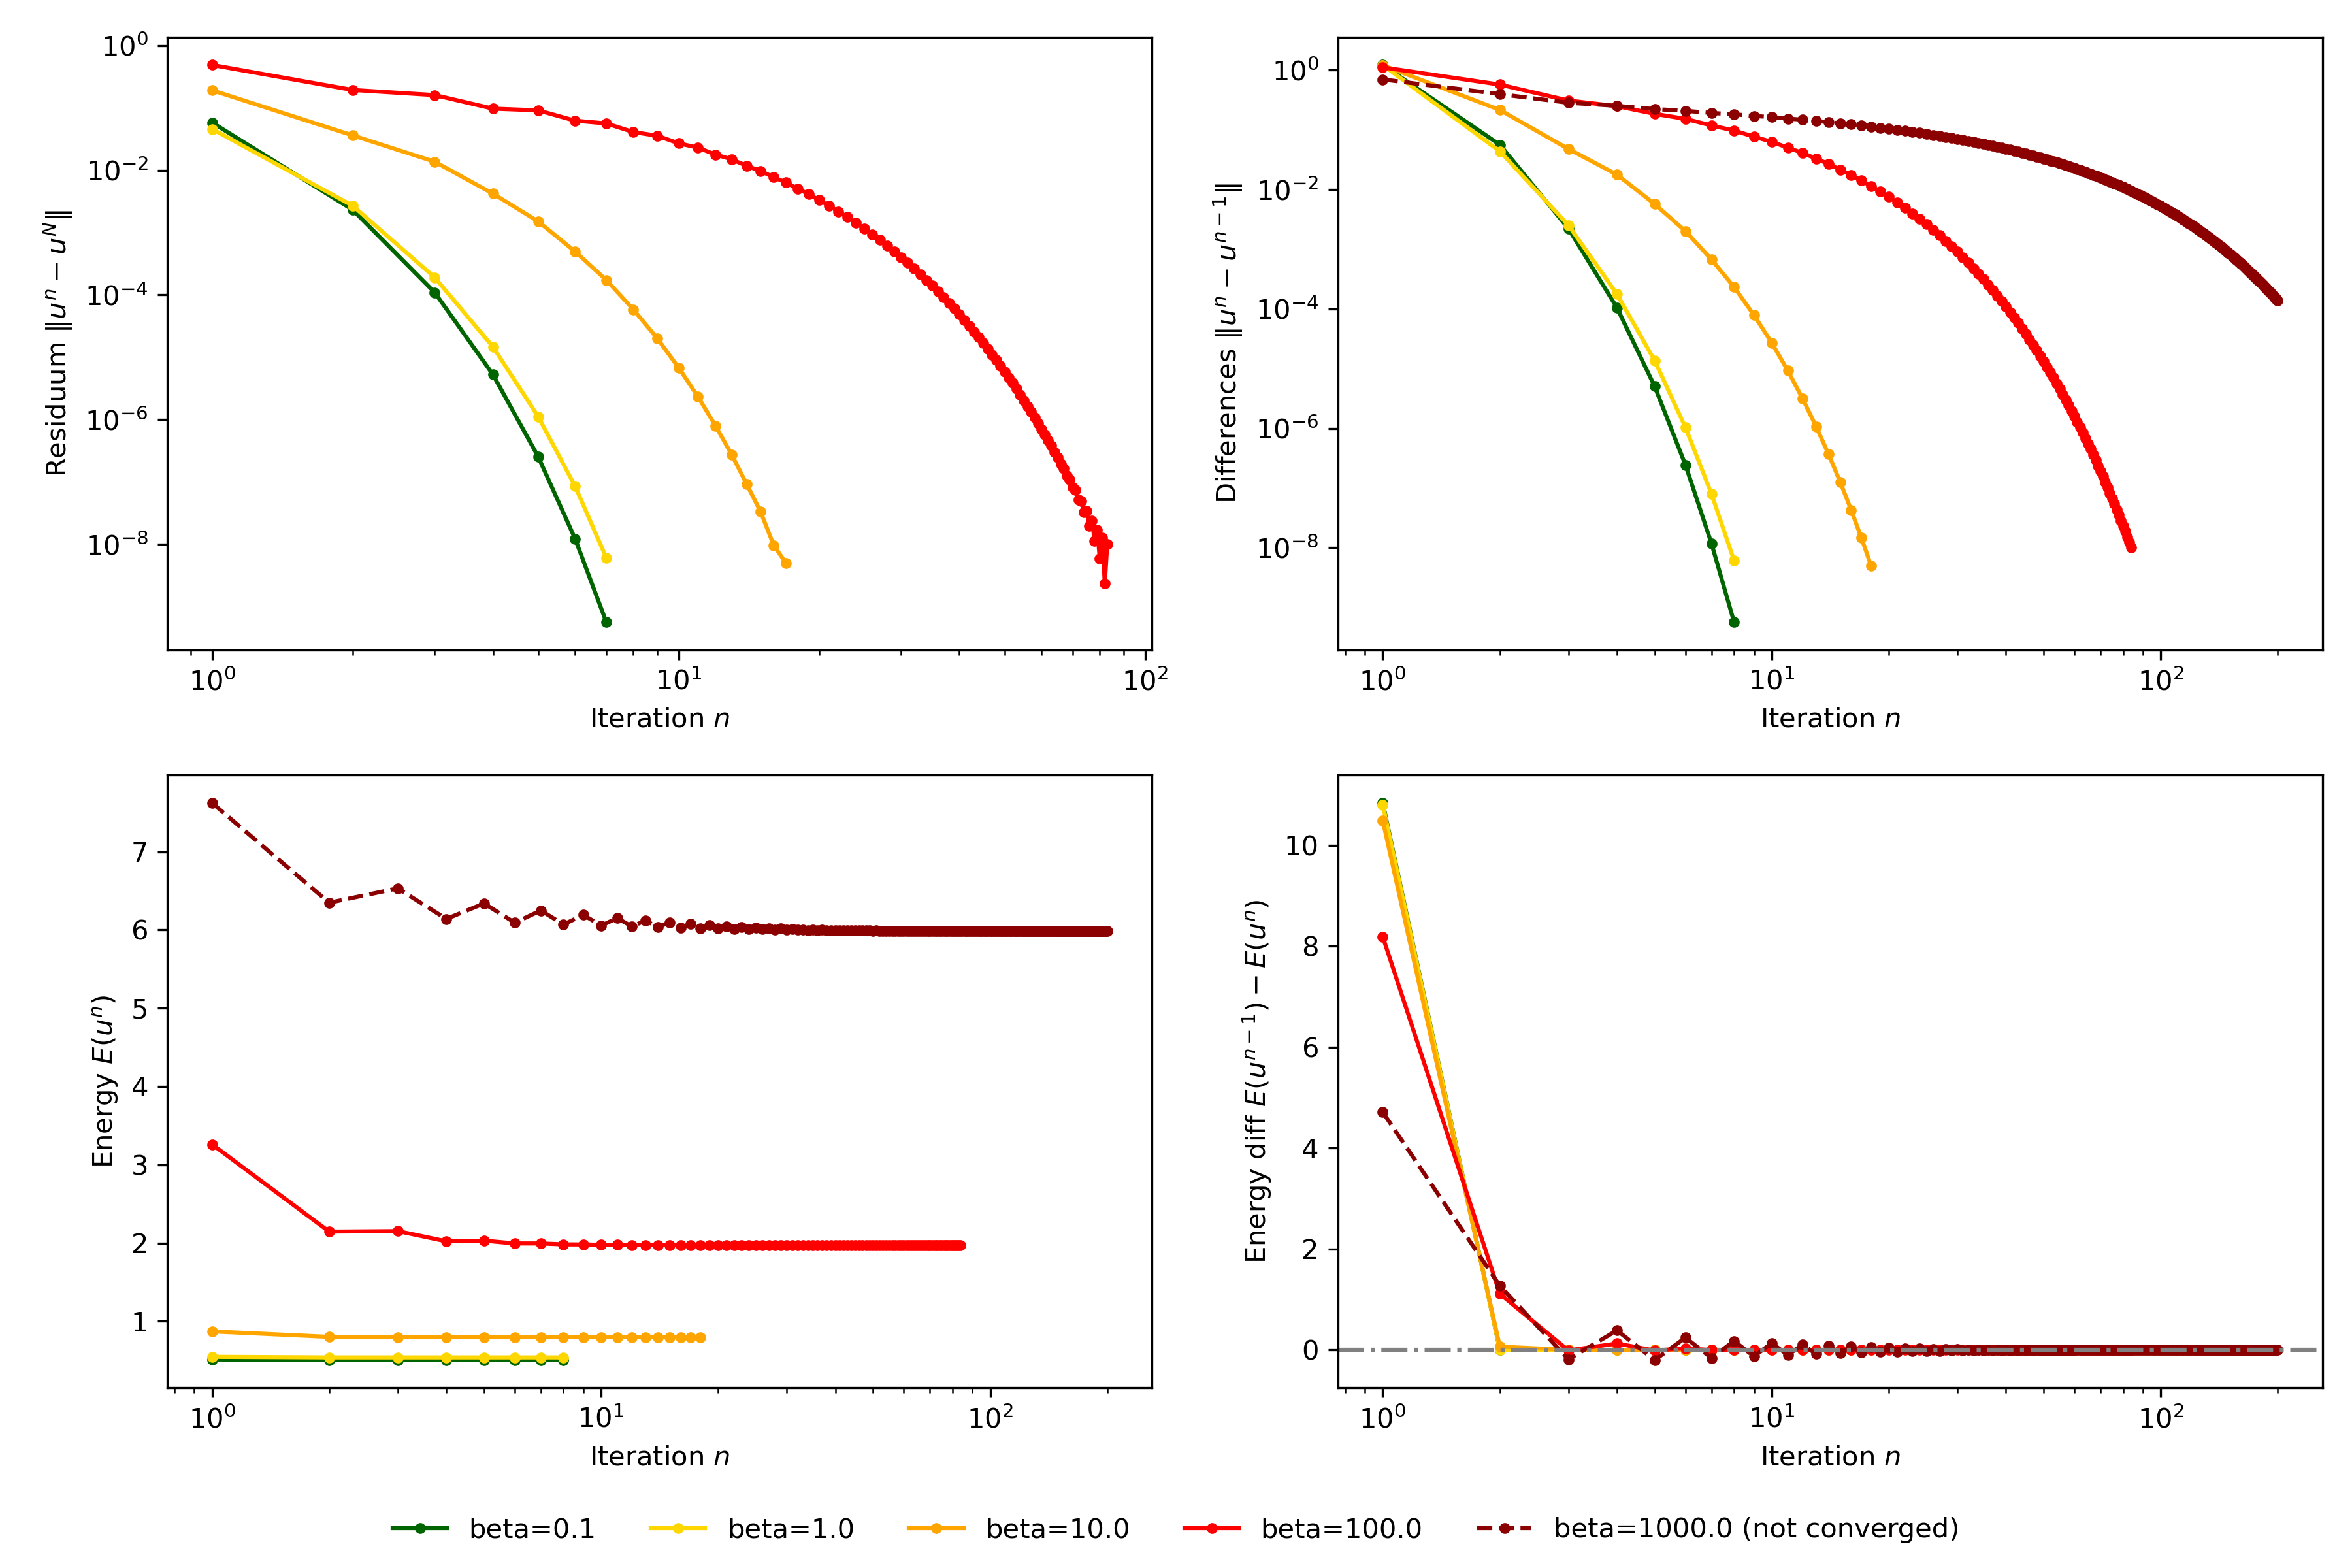
\includegraphics[width=\textwidth]{../img/gpe-inverse-iteration-shifted.png}
	\caption{Die geshiftete Variante der A-Methode.}
\end{figure}

\section{Fazit}

Die A-Methode stellt eine sinnvolle Generalisierung der Inversen Iteration
aus der numerischen Linearen Algebra für nichtlineare Eigenwertprobleme 
der Form $A(v)v = \lambda v$ dar.
Sie kann genutzt werden, um das kleinste Eigenpaar $(\lambda_1, u)$ zu berechnen,
wenn ein echter Abstand zum zweitkleinsten Eigenwert $\lambda_2$ vorliegt, d.h.
$\lambda_1 < \lambda_2$.

\medskip

Die Funktionsweise ist ähnlich zur klassischen Inversen Iteration,
das Problem wird nur
zusätzlich an der Stelle $v$ durch $A(v)$ linearisiert.
Die Konvergenzeigenschaften der A-Methode sind ebenfalls ähnlich, lokal
konvergiert das Verfahren asymptotisch mit $\frac{\lambda_1}{\lambda_2}$
für alle Startwerte $u_0 \in \Honez$ aus einer Umgebung der optimalen Lösung $u$.

Des Weiteren kann eine gedämpfte Version des Verfahrens konstruiert werden,
welche für alle Dämpfungsparameter
$\tau_n \in (0, 2(1 + \frac{\lambda_1}{\lambda_2})^{-1})$
und für alle Startwerte $u_0 \in \Honez$ gegen die Lösung $u$
konvergiert. Insbesondere konvergiert damit auch der Spezialfall $\tau_n = 1$, d.h.
das ungedämpfte Verfahren. Dieser Spezialfall bietet tatsächlich auch lokal
die beste Konvergenzrate, was bedeutet, dass das gedämpfte Verfahren
in zwei Schritte unterteilt werden kann. Im ersten Schritt werden mithilfe
eines Liniensuchverfahrens die optimalen Schrittweiten $\tau_n$ bestimmt,
ist man nahe genug an einer Umgebung der optimalen Lösung, wird die adaptive
Schrittweitensteuerung ausgeschaltet und geht in das ungedämpfte Verfahren
über.

\medskip

So bietet die A-Methode eine interessante Möglichkeit die klassische Inverse
Iteration zu verallgemeinern, hat jedoch auch ihre Schwächen. Insbesondere
reagiert sie im Allgemeinen sehr schlecht auf Shifts. Versuche, die A-Methode
durch eine bessere Linearisierung von $A$ zu verbessern, führen dann
schnell zur eng verwandten J-Methode, welche auch deutlich besser auf Shifts
reagiert und die überlegene Methode darstellt.

\printbibliography

\newpage

\end{document}
